\chapter{Requirements}\label{chapter:requirements}

\section{Project Development Methodology}

Before delving into requirements analysis, it was important to decide upon a project development methodology, since the approach taken to gather the requirements differs according to the methodology chosen.

After some consideration (discussed in appendix~\ref{appendix:methodology}), it was decided that the approach should be a hybrid one of Waterfall and Agile. The project would begin with a strong set of requirements and there would be some up front design for parts of the project that are unlikely to change, such as the database schema. At the implementation stage, the project would switch to a test-driven approach that utilises the best of the agile processes.

\section{Roles}

Simple ODR platforms targeted towards e-commerce disputes typically involve just a buyer and a seller. Our ODR platform is intended to be applied to more serious cases and thus has four main roles:

\begin{itemize}
\item \textbf{Law Firm} - registered to the system by an authorised individual (such as managing director). A Law Firm can have many Agents.
\item \textbf{Agent} - a lawyer, working on behalf of a Law Firm. An Agent must be in one Law Firm.
\item \textbf{Mediation Centre} - a company specialising in the mediation of disputes. A Mediation Centre can have many Mediators.
\item \textbf{Mediator} - working on behalf of a Mediation Centre. A Mediator must be in one Mediation Centre.
\end{itemize}

\section{Use cases}

A good place to begin was to create various use case diagrams representing the roles in the system and the actions they ought to be able to perform. By doing so, it would also be possible to derive common classes and actions by examining similar or duplicating use case scenarios. These use cases were derived from early meetings with the customer and other stakeholders.

\subsection{Registration}

\begin{figure}[h!]
  \centering
    \ifimages
    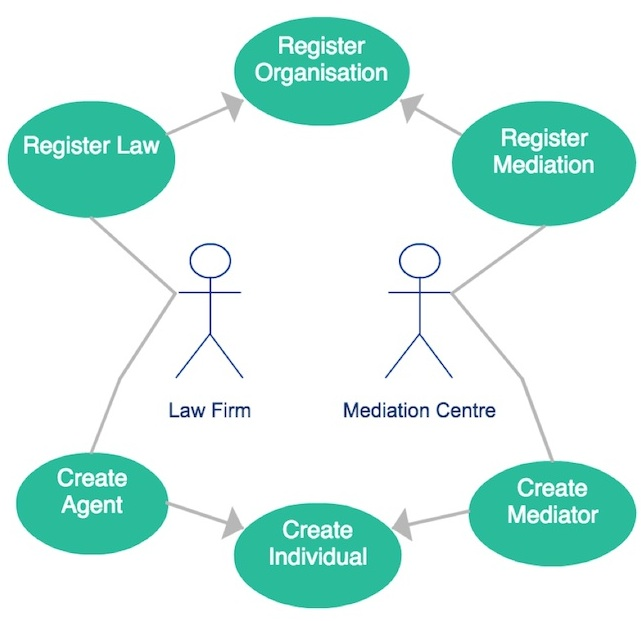
\includegraphics[width=0.7\textwidth]{use_case--registration}
    \fi
  \caption{Use case diagram showing registration feature}
  \label{uml:useCase:registration}
\end{figure}

Authorised individuals should be allowed to register accounts representing their company (be it a law firm or mediation centre), and within that organisation account they should be able to register individual accounts. These individual accounts should be agents or mediators depending on the organisation type.

Figure~\ref{uml:useCase:registration} shows this in terms of the law firms and mediation centres. A generalised action has been added in both the organisation and individual registration, showing where it might be possible to use a common class or database table to accomplish both goals.

\subsection{Disputes}

\begin{figure}[h!]
  \centering
    \ifimages
    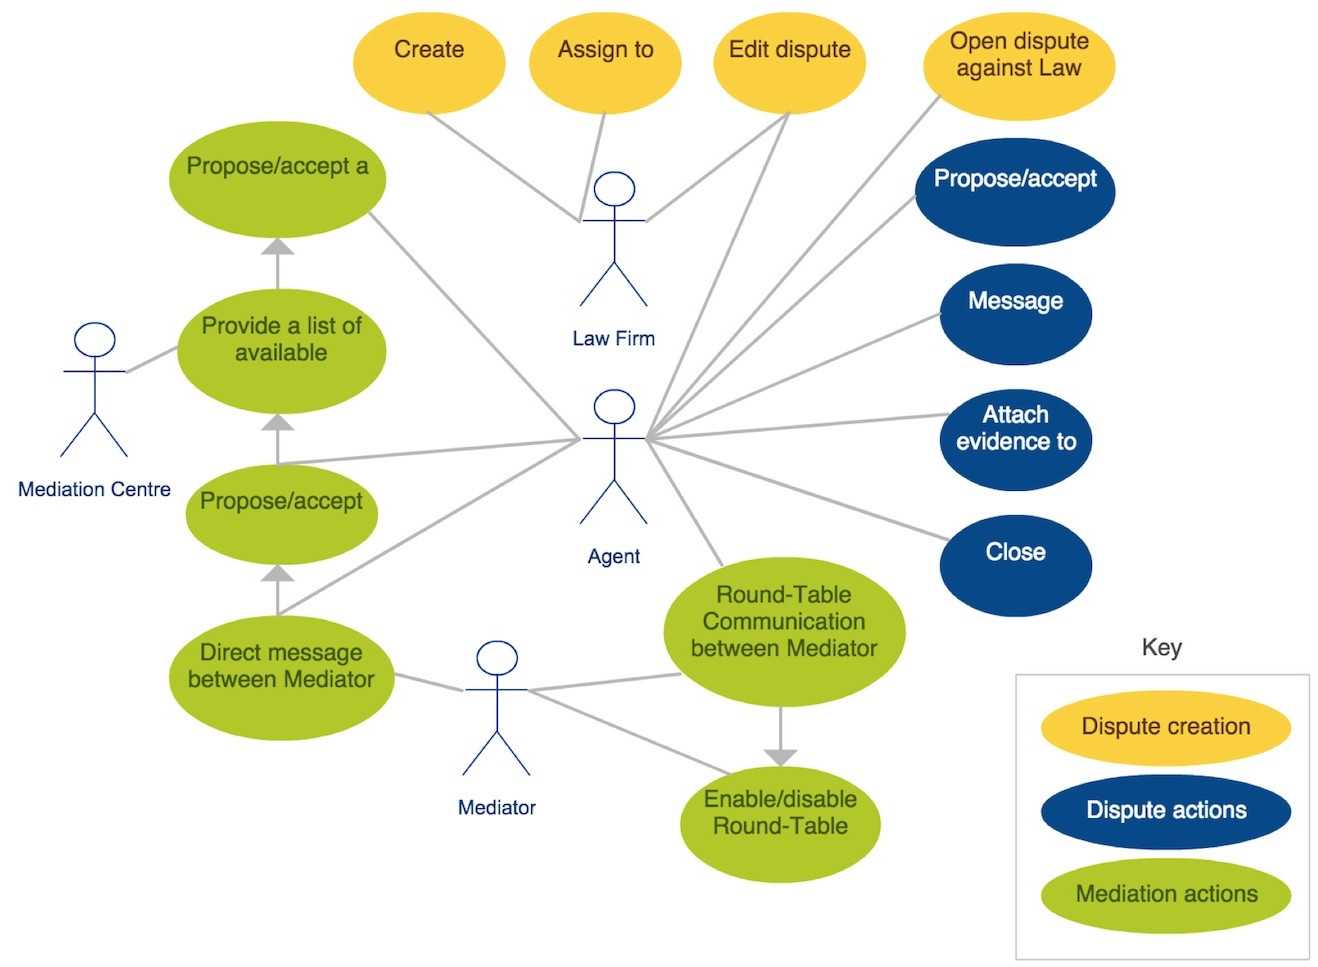
\includegraphics[width=\textwidth]{use_case--disputes}
    \fi
  \caption{Use case diagram showing actions available in a dispute}
  \label{uml:useCase:disputes}
\end{figure}

Figure~\ref{uml:useCase:disputes} shows the roles and actions involved in the creation, mediation and closing of a dispute. Arrows denote where one action has a dependency on another.

Only law firms can create new disputes. There is then some back-and-forth assignment between law firms and agents until both sides of a dispute are represented by opposing agents. This is identified as the `dispute creation' stage.

Inside a dispute, agents should be able to negotiate the dispute lifespan, exchange messages and evidence, and be able to close the dispute. In a best-case scenario, this is all that is required to successfully resolve a dispute. This is known as the `dispute' stage.

Should it be required, an agent can propose mediation, and there is a defined process of administration between the agents and mediation centre required to get the dispute `in mediation'. Once in this state, the agents can communicate only through the mediator, unless the mediator feels the dispute is close to resolution and decides to enable round-table communication.

\subsection{Miscellaneous}

\begin{figure}[h!]
  \centering
    \ifimages
    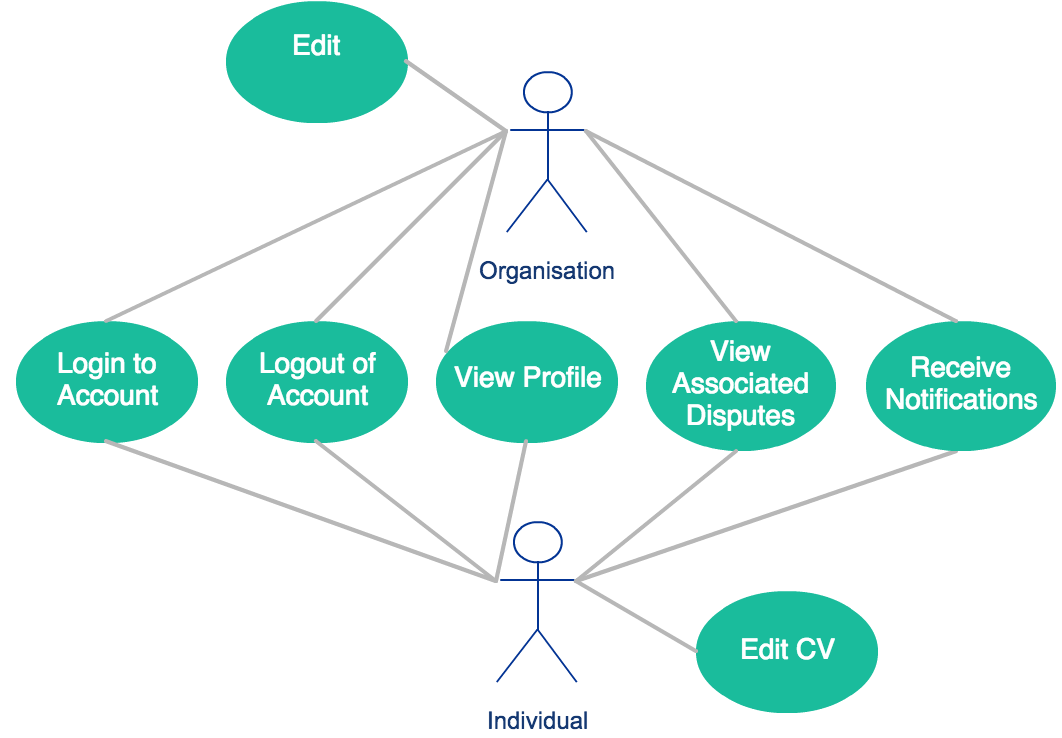
\includegraphics[width=0.95\textwidth]{use_case--miscellaneous}
    \fi
  \caption{Use case diagram demonstrating other miscellaneous requirements}
  \label{uml:useCase:miscellaneous}
\end{figure}

Other, lesser elements of functionality are shown in the miscellaneous use case diagram in figure~\ref{uml:useCase:miscellaneous}. For example, agents should be able to peruse a mediator's CV before making a decision as to which mediator to opt for; this suggests the need for a ``view profile" facility with custom fields for the CV, which could be as simple as a HTML textarea or as complicated as an integrated PDF uploader and viewer. Given the tight deadline of the project and the scale of the system, it was decided that these miscellaneous features should be kept as simple as possible.

\section{Dispute process}

Although the use case diagrams describe the features required by the system, they do not make it very clear when those features should or should not be available. An early meeting with the customer emphasised that a dispute should follow a very specific workflow.

\begin{figure}[h!]
  \centering
    \ifimages
    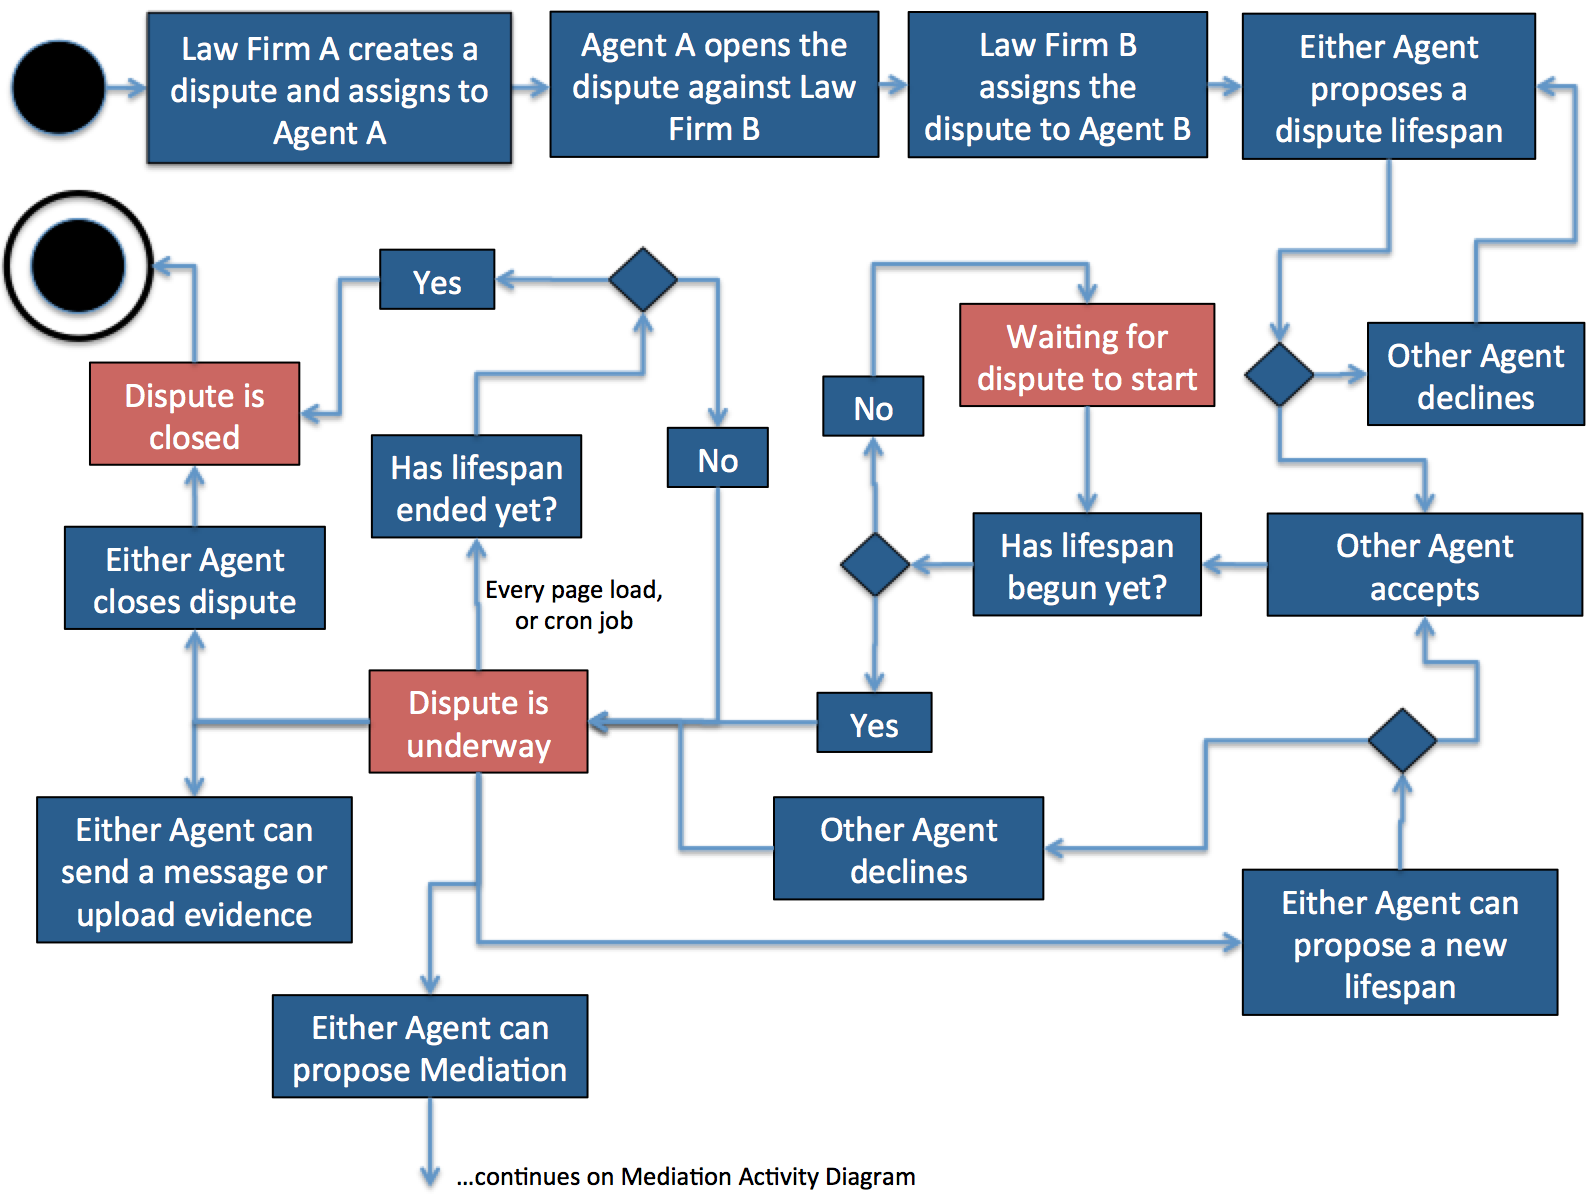
\includegraphics[width=\textwidth]{dispute_process}
    \fi
  \caption{Activity diagram showing the workflow required in creating a dispute}
  \label{uml:activity:dispute}
\end{figure}

The activity diagram in figure~\ref{uml:activity:dispute} shows the creation of a dispute and the features that become available to the agents when the dispute has been initialised. The activity diagram continues into figure~\ref{uml:activity:mediation}, which shows what is involved in putting a dispute into mediation. In both diagrams, red boxes indicate the current `state' of the dispute.

\begin{figure}[h!]
  \centering
    \ifimages
    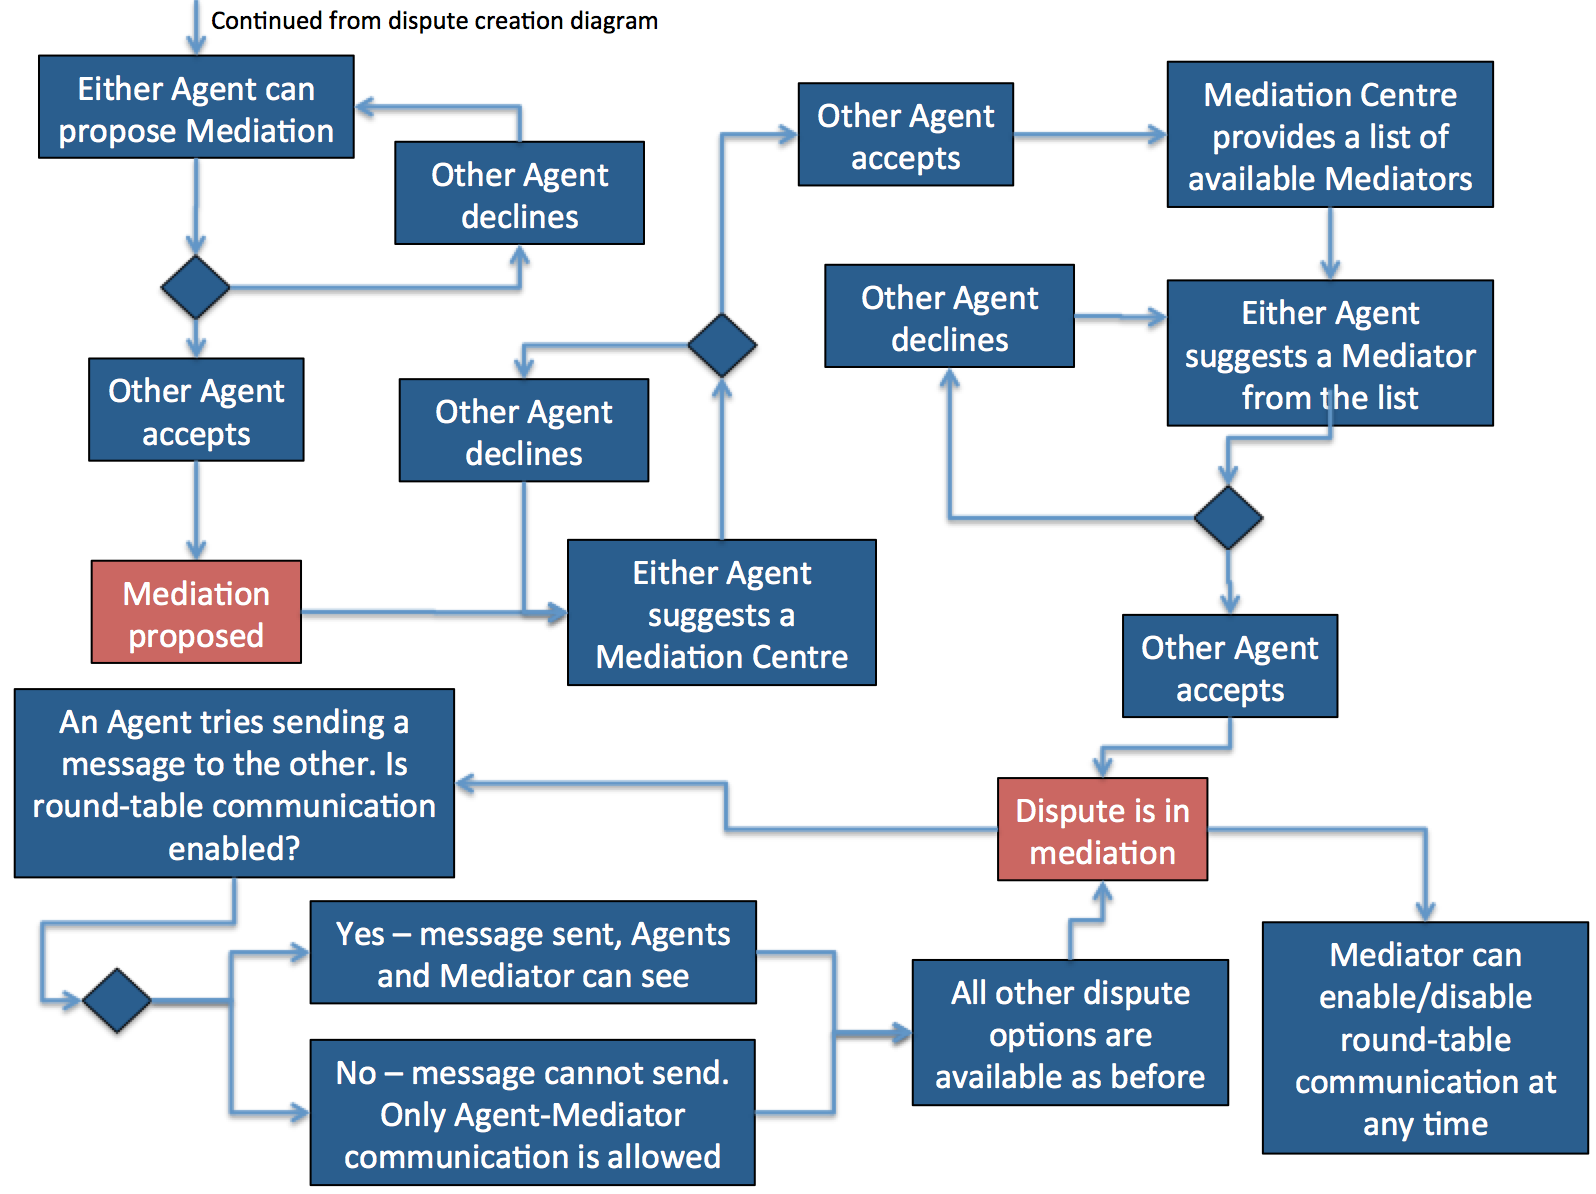
\includegraphics[width=\textwidth]{dispute_process--mediation}
    \fi
  \caption{Activity diagram showing the workflow involved in getting a dispute into mediation}
  \label{uml:activity:mediation}
\end{figure}

Through the requirements-gathering process it became clear that the end-to-end lifecycle of even a simple dispute is actually quite complicated. I later developed a webpage, ``How does SmartResolution work?", to help explain the process of a dispute. The complete workflow can be found in appendix~\ref{appendix:workflow}. If the dispute-creation or mediation process is still unclear, it is recommended that you read and understand the contents of appendix~\ref{appendix:workflow} before continuing.

\section{Features}

Following on from the use case diagrams, it was critical to explicitly define the project requirements in a textual way. In a traditional Waterfall model, a requirements specification is a key deliverable created at the beginning of the process, whereas in an agile model, features are represented as user stories which are then estimated, prioritised and tackled iteratively. My approach to textualising requirements is a compromise between plan-driven and agile approaches. In this project I specified requirements in the form of Cucumber features, which are executable in a BDD way that lends itself perfectly to the agile practices of TDD and CI.

BDD, or business-driven development, allows you to write executable features in a human-readable way so that a business analyst is able to understand the requirements but does not need to know the technical implementation. The features follow a convention known as the Gherkin syntax so that each feature step can be matched to a corresponding step definition represented in code, allowing automated end-to-end testing.

Appendix~\ref{appendix:requirements} contains the full set of Cucumber features which were originally signed off; these features act as the requirements specification. The nature of these being a part of the codebase means that they can evolve over time, which is simultaneously an advantage (for always being in line with the implementation) and a disadvantage (for allowing ``requirements creep"). As a result, the Cucumber features at the end of the project are now markedly different to the original set of signed-off features. Though these current features could also have been included in the appendix, they only represent the features at the time of publication and are likely to change should this project be developed further in future. Given that there is little historical value in this, I have decided not to include the current set of Cucumber features in the appendix. For the most up-to-date Cucumber features, please refer to the technical hand-in or to the GitHub repository.

\section{Development Methodology versus Project Management}

Each of the development methodologies discussed has an associated project management approach. Waterfall projects tend to use Gantt charts to plan progress, whereas agile approaches tend to use sprints to plan individual iterations. As this project would be using a hybrid development methodology, the question was raised as to whether or not it should be using a hybrid project management approach.

Given that the first half of the project would be plan-driven and that significant efforts were made in the early stages of the project to clarify exact requirements, it made sense to adopt the plan-driven approach of creating a Gantt chart which plans out the implementation of the features.

\begin{figure}[h!]
  \centering
    \ifimages
    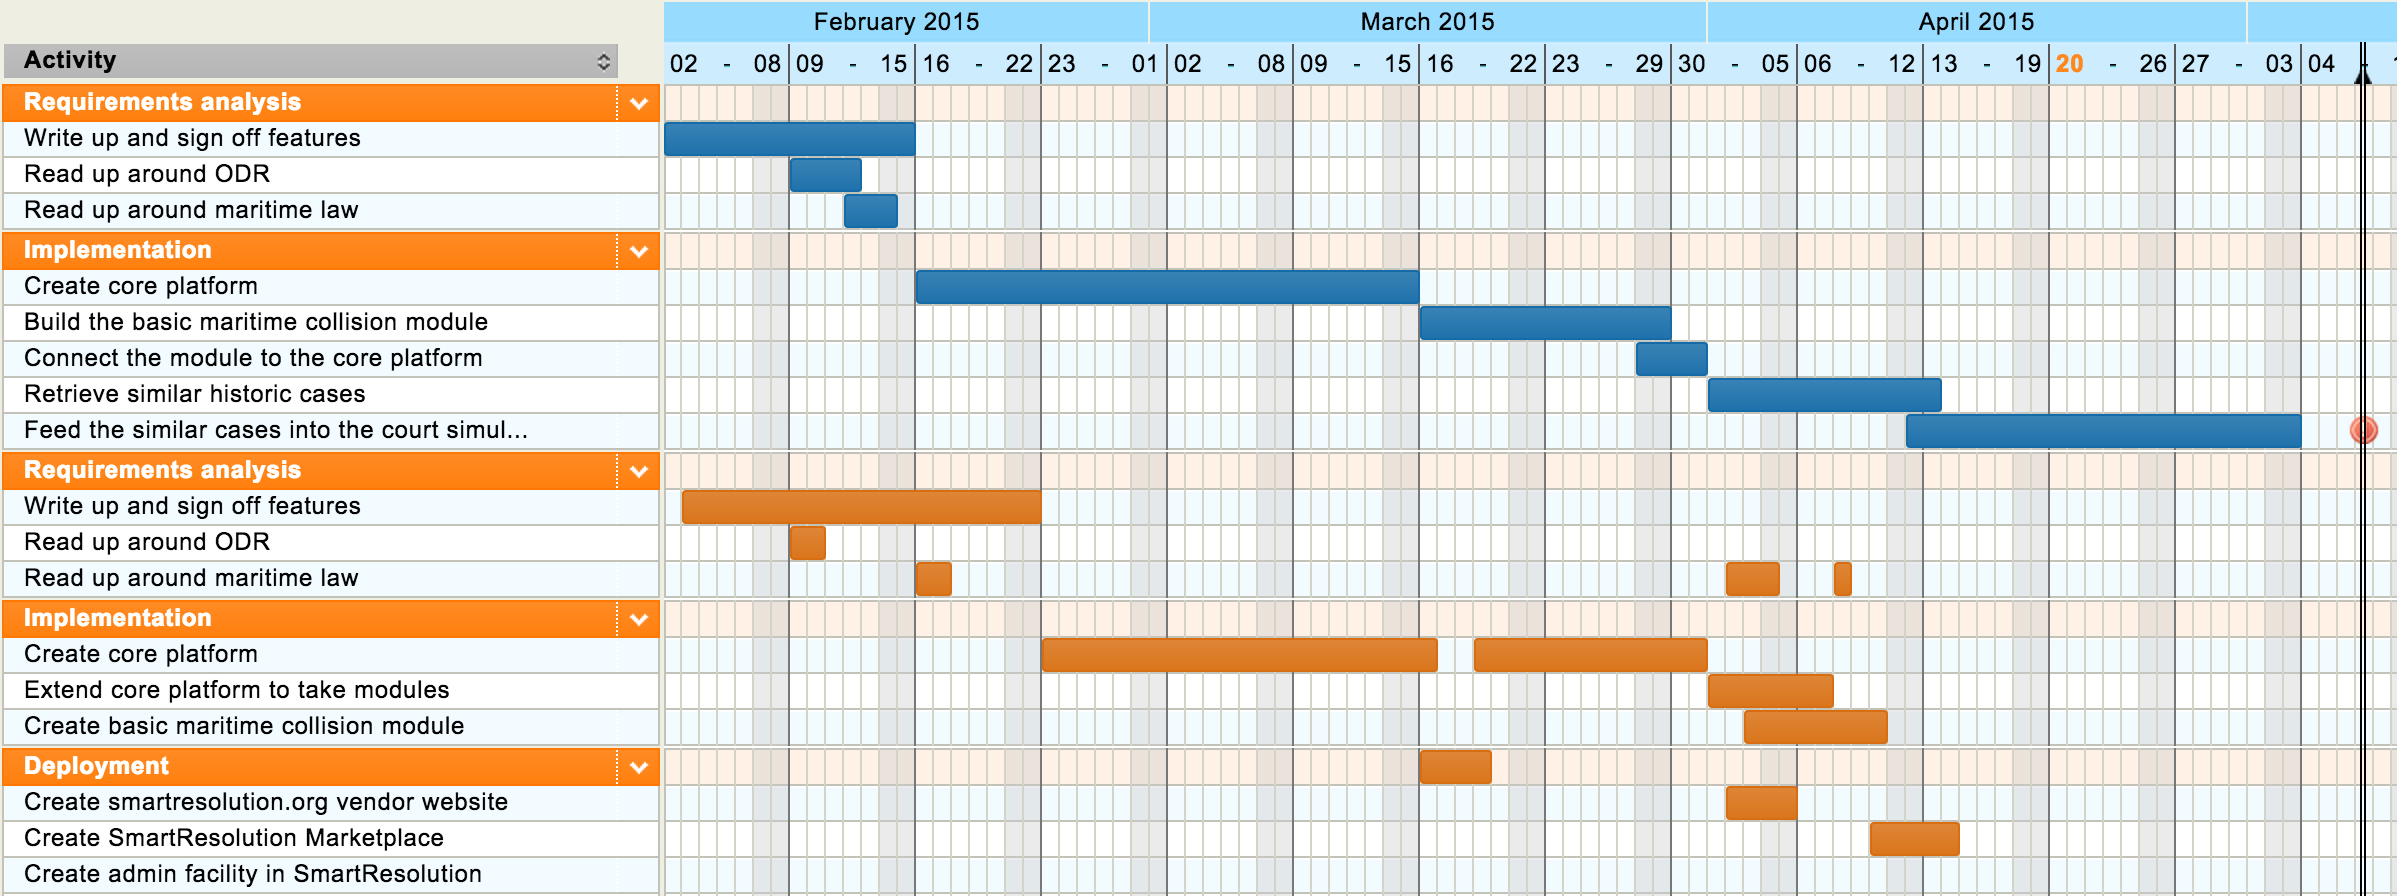
\includegraphics[width=1.4\textwidth,angle =90]{gantt}
    \fi
  \caption{Gantt chart showing the original plan, compared with the plan actually followed}
  \label{uml:gantt}
\end{figure}

The Gantt chart in figure~\ref{uml:gantt} shows two timelines. The time periods in blue represent the original Gantt chart I intended to follow for this project. The time periods in orange represent what actually happened over the course of the project. The reasons for the disparities between the two are discussed in section~\ref{section:timeManagement}.

\section{SmartResolution}

The report thus far has discussed the project in the form of two main components: the core ODR platform and the maritime collision module. Realistically, a third component was required: a vendor website. This website would host the core software and provide instructions on how to install it onto a server.

If developers were to be excited enough about ODR to develop modules of functionality like the maritime collision module, then this project would require a brand. I felt that the term `SmartResolution' embodied what the ODR platform was all about: online dispute resolutions done in a smart way, by interpreting disputes using artificial intelligence to automatically suggest resolutions. SmartResolution is the term I'll use to refer to the core platform from this point onwards.

Far from being just an information resource, the SmartResolution website would later provide a facility to download and install SmartResolution modules directly through the SmartResolution installation itself, a little like downloading an app to an Android device directly through the Google Play store. The `SmartResolution Marketplace' was implemented towards the end of the project.